
%(BEGIN_QUESTION)
% Copyright 2012, Tony R. Kuphaldt, released under the Creative Commons Attribution License (v 1.0)
% This means you may do almost anything with this work of mine, so long as you give me proper credit

A 15 pound weight hangs from the ceiling, suspended from two equal-length strings.  The angle of each string is 50$^{o}$ from horizontal:

$$\includegraphics[width=15.5cm]{i02586x01.eps}$$

Calculate the amount of tension in each string.  Hint: because the strings are equal length and have equal angles with respect to horizontal, the tension in each string will likewise be equal.

\vskip 10pt

$F_{tension}$ = \underbar{\hskip 50pt} lbs

\vskip 20pt \vbox{\hrule \hbox{\strut \vrule{} {\bf Suggestions for Socratic discussion} \vrule} \hrule}

\begin{itemize}
\item{} Perform a ``thought experiment'' where you imagine the angles in this problem approaching 90$^{o}$ (i.e. vertical strings).  What happens to the tension within each string as they become more vertical?
\end{itemize}

\underbar{file i02586}
%(END_QUESTION)





%(BEGIN_ANSWER)

$F_{tension}$ = {\bf 9.791 lbs} (in \underbar{each} string)

%(END_ANSWER)





%(BEGIN_NOTES)


%INDEX% Mathematics review: trigonometric calculations

%(END_NOTES)


